\documentclass[10pt]{beamer}

\usetheme{metropolis}
\usepackage{appendixnumberbeamer}

\usepackage[backend=bibtex]{biblatex}

\usepackage{booktabs}
\usepackage[scale=2]{ccicons}

\usepackage{pgfplots}
\usepgfplotslibrary{dateplot}

\usepackage{xspace}
\newcommand{\themename}{\textbf{\textsc{metropolis}}\xspace}

\usepackage{biblatex}
\addbibresource{demo.bib}
\renewcommand{\bibname}{}

\usepackage{CJKutf8}

\title{Summer Camp of Westlake University}
\subtitle{Who Am I, Where Did I Come From, Where Am I Going}
\date{June 30, 2024}
\author{Yanchen Huang}
\institute{Nanjing University Software Institute}
% \titlegraphic{\hfill
\includegraphics[height=1.5cm]{logo.pdf}}

\begin{document}

\maketitle

\begin{frame}{Table of contents}
  \setbeamertemplate{section in toc}[sections numbered]
  \tableofcontents[hideallsubsections]
\end{frame}

\section{Academic background}

\begin{frame}[fragile]{Personal Information}
    \begin{columns}
        \column{0.3\textwidth}
            \begin{figure}
            \centering
            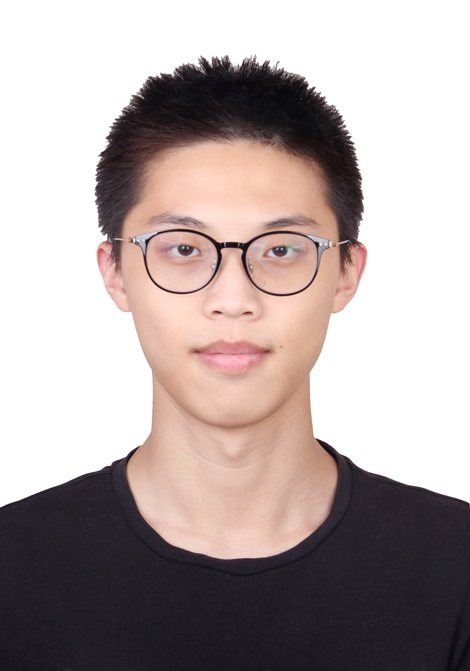
\includegraphics[width=\textwidth]{pic/photo_2_resize.jpg}
            \caption{My Photo}
            \end{figure}
        \column{0.7\textwidth}
            \begin{itemize}
                \item \textbf{My Major:} Software Engineering
                \item \textbf{My Rank:} 47 / 257
                \item \textbf{My GPA:} 4.44 / 5.00
                \item \textbf{Score of CET6:} 536
                \item \textbf{Main courses}
            \end{itemize}
               \begin{table}[]
	\centering
	\begin{tabular}{ll}
		\hline
		\textsc{Course} & \textsc{Grade} \\ \hline
		    Data Structure and Algorithm Analysis   &  91     \\ \hline
		  Software Engineering and Computing     &   95    \\ \hline
            Computer Operating Systems     &   92    \\ \hline
            Software Testing     &   97    \\ \hline
            Human-Computer Interaction Systems     &   95    \\ \hline
	\end{tabular}
	\label{tab:my-table}
\end{table}
        \end{columns}
\end{frame}

\begin{frame}[fragile]{Major Awards}
\begin{itemize}
    \item 2022.06.08 \textbf{EL Programming Competition}, Third Prize
    \item 2022.12.05 \textbf{Social Pratice of Nanjing University}, Excellent Student
    \item 2022.12.15 \textbf{The People's Scholarship}, Second Prize
    \item 2023.12.13 \textbf{The People's Scholarship}, Third Prize
\end{itemize}
\end{frame}

\section{Research Experience}
\begin{frame}[fragile]{AI Couplet}
\begin{itemize}
    \item The first time to contact with AI
    \item A preliminary understanding of the \textbf{NLG} task
    \item The learning of the \textbf{RNN, LSTM} model
\end{itemize}
\begin{figure}
    \centering
    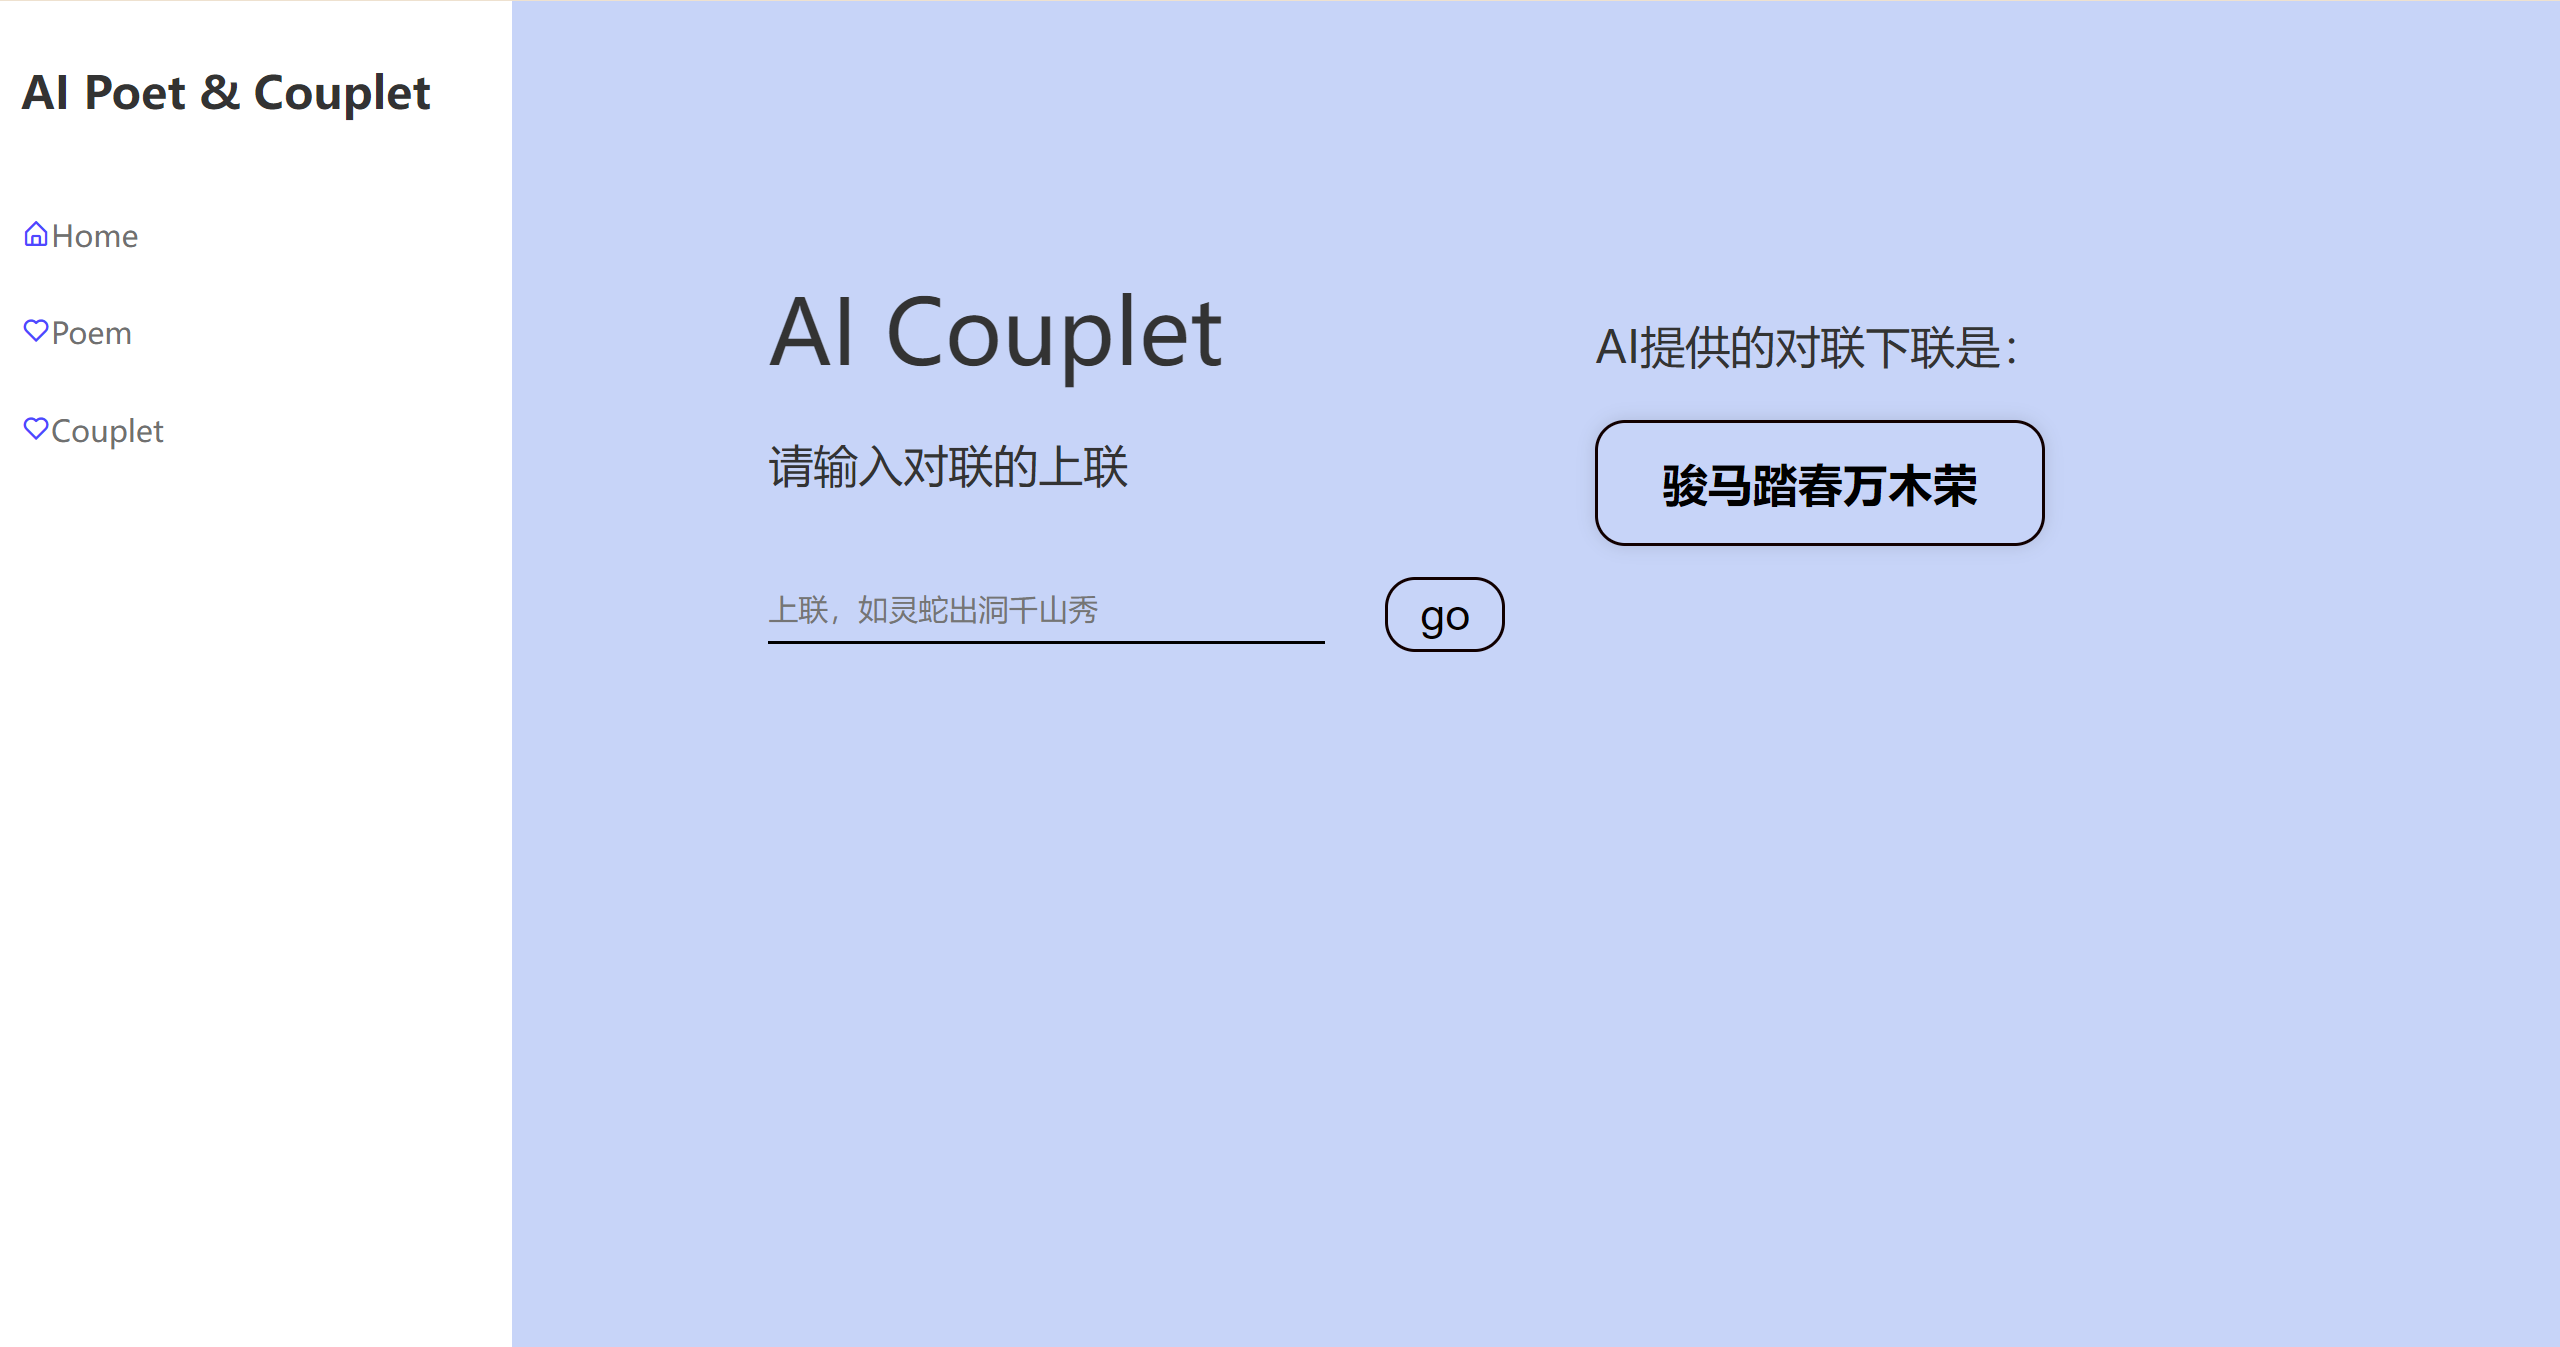
\includegraphics[width=0.8\textwidth]{pic/ai_couplet.png}
    \caption{The homepage of AI Couplet project}
    \label{fig:my_label}
\end{figure}
\end{frame}

\begin{frame}[fragile]{Fake News Judgment}
I Participate in the summer camp of the NLP lab of Nanjing University and choose the subject of social media computing, mainly for the \textbf{fake news Judgment}.

The research process:
\begin{itemize}
    \item Paper Reading
    \item Research Plan
    \item Data Collecting, filtering and analysis
    \item Model Running
    \item Error Study
    \item Case Study
\end{itemize}
\end{frame}

\begin{frame}{Fake News Judgment}
Fake news judgment is essentially a classification task. After reading 8 papers concerning the fake news and the methods of classification such as \textbf{TextCNN}\cite{TextCNN} and \textbf{BERT}\cite{BERT}, we worked out the experiment plan together.

Since most fake news judgments in the papers are based on English texts, to conduct this task, we used the Weibo datasets of size 4771.
We analysis these data according to the \textbf{BWS}(Best-Worst-Scaling)\cite{BWS}.
\end{frame}

\begin{frame}{Fake News Judgment}
The process of Best-Worst-Scaling is below:
\begin{itemize}
    \item Divide the items to be labeled into multiple 4-grams.
    \item For each n-gram, annotators are asked to select the item that best and least matches the target attribute. This design enables the pairwise comparison results of five pairs of six items in each n-tuple to be obtained through a single annotation.
    \item Each item is scored using a counting method: the number of times an item was selected as the "most appropriate" choice minus the number of times it was selected as the "least appropriate" choice, with a score ranging from -1 to 1.
\end{itemize}
\end{frame}

\begin{frame}{Fake News Judgment}
    \begin{columns}
        \column{0.5\textwidth}
        \begin{figure}
            \centering
            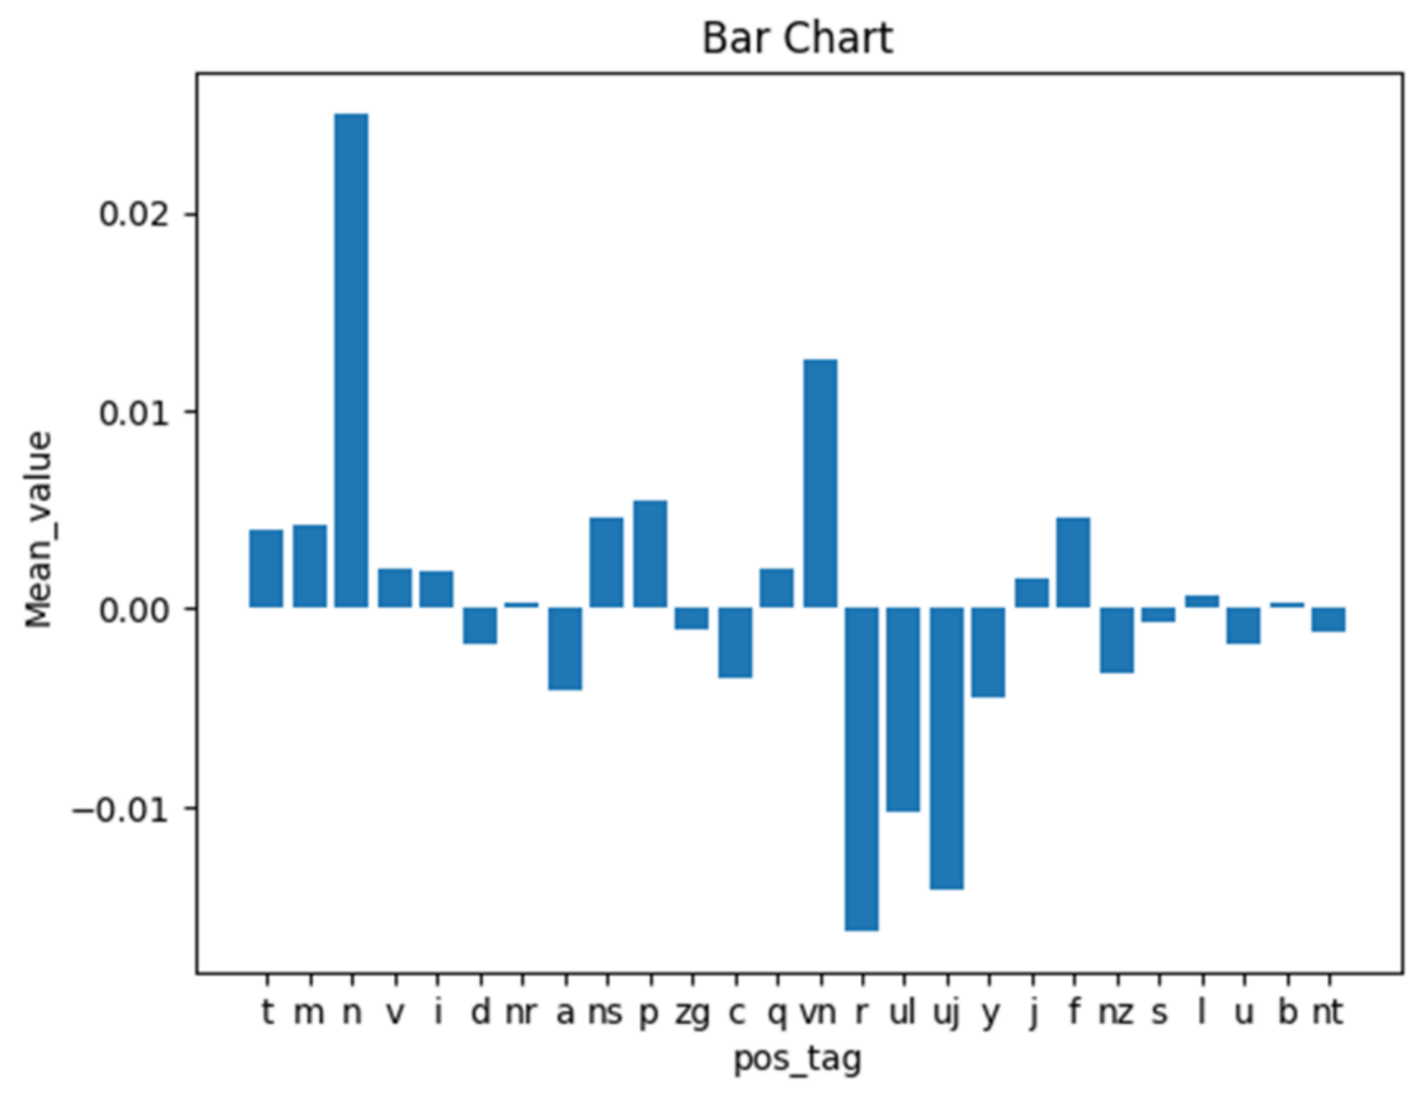
\includegraphics[width=0.9\textwidth]{pic/pos_analysis.png}
            \caption{The pos anallysis of data}
            \label{fig:my_label}
        \end{figure}
        \column{0.5\textwidth}
        \begin{figure}
            \centering
            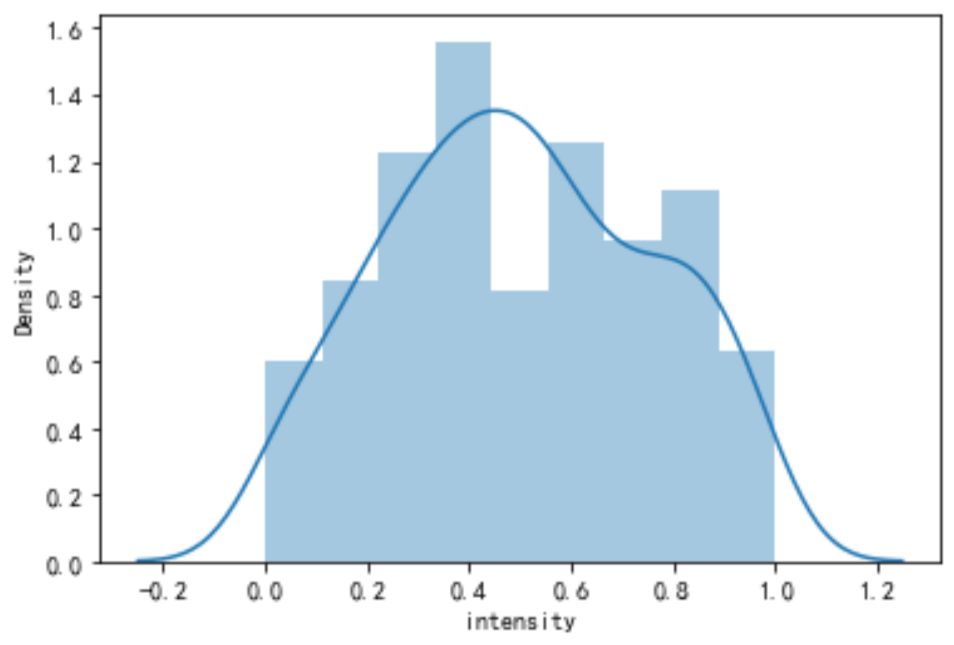
\includegraphics[width=\textwidth]{pic/bws_res.png}
            \caption{The result of the BWS label}
            \label{fig:my_label}
        \end{figure}
    \end{columns}
\end{frame}

\begin{frame}{Fake News Judgment}
The final results in \textbf{LSTM}, \textbf{TextCNN} and \textbf{BERT} are shown below. Convert the text into a sequence and pad it to the same length, do embedding to encode each sequence into a vector representation. Then train the classification model.
\begin{table}[]
	\centering
	\begin{tabular}{|l|l|l|l|l|}
		\hline
		\textbf{Model}   & \textbf{Acc}   & \textbf{Pre}   & \textbf{Rec}   & \textbf{F1}    \\ \hline
		LSTM    & 0.781 & 0.778 & 0.768 & 0.773 \\ \hline
		TextCNN & 0.839 & \textbf{0.828} & 0.835 & 0.833 \\ \hline
		BERT    & \textbf{0.853} & 0.792 & \textbf{0.957} & \textbf{0.867} \\ \hline
	\end{tabular}
	\label{tab:my-table}
\end{table}
\end{frame}

\begin{frame}{Fake News Judgment}
\begin{itemize}
    \item How to read papers? How to help the current subject?
    \item How to do the data analysis? Pos analysis, Correlation test
    \item How to design the experiment? Cross Domain, Feature Selection
\end{itemize}
\end{frame}

\begin{frame}[fragile]{Chinese Idiom Error Detection}
Although Chinese idioms are widespread, idioms have non-compositionality and specific semantic or grammatical
properties, resulting in the idioms in isolation being often unintelligible without additional explanation. Neglecting
these properties will lead to the problem of idiom misuse. 

What I did in this subject:
\begin{itemize}
    \item Baseline Models —— \textbf{K\_BERT}\cite{KBERT}
    \item \textbf{LLMs}(Large Language Models) performance
    \item CEE datasets expanding
\end{itemize}
\end{frame}

\begin{frame}{Chinese Idiom Error Detection}
Create knowledge triples of idioms and their interpretations to embed into the model.
\metroset{block=fill}
\begin{exampleblock}{Interpretation}
\begin{CJK}{UTF8}{gbsn}
白玉微瑕:比喻很好的人或物有些小缺点,美中不足。
\end{CJK}
\end{exampleblock}
\begin{alertblock}{Triple}
\begin{CJK}{UTF8}{gbsn}
(白玉微瑕, ,比喻很好的人或物有些小缺点,美中不足。)
\end{CJK}
\end{alertblock}
\end{frame}

\begin{frame}{Chinese Idiom Error Detection}
\begin{figure}
\centering
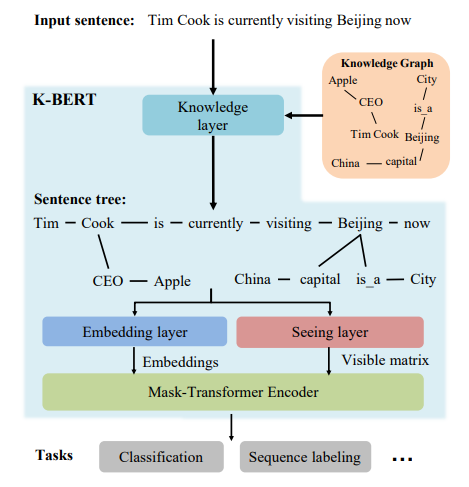
\includegraphics[width=0.6\textwidth]{pic/KBERT.png}
\caption{K-BERT\cite{KBERT}}
\label{fig:my_label}
\end{figure}
\end{frame}

\begin{frame}{Chinese Idiom Error Detection}
In order to test the performance of the large language models on the idiom error detection task, a prompt is designed below:
\metroset{block=fill}
\begin{alertblock}{Prompt}
\begin{CJK}{UTF8}{gbsn}
你是一名精通中国成语的语言学者,现在需要你完成成语纠错任务,任务描述如下:你的输入是一个字符串文本,你首先需要理解字符串文本的语义,然后你要识别出字符串文本中所包含的成语,然后你要根据成语的释义判断在这个字符串中成语是否被正确使用。最后以字典形式返回判断结果。你只需要给出最终判断结果,不需要给出解释。
请参照下面的例子进行输入输出:
输入:这条小河看上去浮光掠影,旁边的树林郁郁葱葱。输出:\{"浮光掠影": false, "郁郁葱葱": true\}
输入: 这家伙办事毫发不爽,小气极了。 输出:\{"毫发不爽": false\}
输入: 发展低碳经济首当其冲的是要坚持节约资源。 输出:\{"首当其冲": false\}
接下来轮到你:
输入: \{input\_text\} 输出:
\end{CJK}
\end{alertblock}
\end{frame}

\begin{frame}{Chinese Idiom Error Detection}
The results in \textbf{K-BERT} and \textbf{LLMs}. Here the \textbf{CLLA}(Cross Layer Levitate Adapter) is the architecture proposed in this subject, 
\begin{table}[]
	\centering
	\begin{tabular}{llll}
		\toprule
		\textbf{Model}  & \textbf{Pre}  & \textbf{Rec}  & \textbf{F1}   \\ \midrule
		K-BERT & 0.829 & 0.753 & 0.789 \\
		CLLA   & \textbf{0.850} & 0.739 & \textbf{0.791} \\ \midrule
        GLM-4 & 0.651 & 0.910 & 0.608 \\
        GPT-4 & 0.524 & 0.821 & 0.507 \\
        GPT-3.5-turbo & 0.628 & 0.400 & 0.391 \\
        Qwen-turbo & 0.576 & 0.839 & 0.541 \\
        Qwen-max & 0.556 & 0.891 & 0.545 \\
        ERNIE-Bot-4 & 0.532 & \textbf{0.968} & 0.552 \\
        baichuan2-13b-chat-v1 & 0.656 & 0.167 & 0.224 \\
        Spark v3.0 & 0.495 & 0.596 & 0.413 \\ \midrule
	\end{tabular}
	\label{tab:my-table}
\end{table}

\end{frame}

\begin{frame}[fragile]{Chinese Idiom Error Detection from another perspective}
Through case analysis of some of the previous experimental results, it is found that most of the idioms in the sentences with wrong interpretations can be detected. However, there are some other cases.
\metroset{block=fill}
\begin{alertblock}{Case One}
\begin{CJK}{UTF8}{gbsn}
这些年轻的科学家决心以无所不为的勇气,探索大自然的奥秘。

老王一句话揭了他的短,惹得他火冒三丈,气冲霄汉。
\end{CJK}
\end{alertblock}
\begin{alertblock}{Case Two}
\begin{CJK}{UTF8}{gbsn}
巧夺天工的大自然刺激了她的感官,也抚慰了她的心灵。

北京电视台的编导很有水平,几个经济类节目都办得绘声绘色。
\end{CJK}
\end{alertblock}
These cases are roughly correct in the interpretations, but errors occur in the \textbf{sentiment} of the idiom and the \textbf{object} of use of the idiom.
\end{frame}

\begin{frame}{Chinese Idiom Error Detection from another perspective}
For \textbf{sentiment}, the regular sentiment analysis method, \textbf{HanLP}\cite{HanLP} or \textbf{UIE}\cite{UIE}, is used to analyze the original sentence and the paraphrase of the idiom to obtain the sentiment score value, and \textbf{the difference value} is used as the sentiment difference. 
\metroset{block=fill}
\begin{exampleblock}{Example}
\begin{CJK}{UTF8}{gbsn}
李师傅被评为模范,同事们来庆贺,好友来闹酒,真是满城风雨。

某一事件(坏)事传播很广,到处议论纷纷,
\end{CJK}
\end{exampleblock}
\begin{alertblock}{Sentiment Result}
Sentence: 0.6435999274253845

Interpretations: -0.19486963748931885

Idiom: 0.45388904213905334
\end{alertblock}
\end{frame}

\begin{frame}{Chinese Idiom Error Detection from another perspective}
For the judgment of consistency of sentence description object and idiom object, it is somewhat complicated. The following methods are tried, but the results are not well.
\begin{itemize}
    \item Through \textbf{dependency syntactic parsing} and \textbf{Semantic Role Labelling}, capture the description object in the sentence. However, many sentences describe objects that do not appear in the sentence.
    \item Define a set of categories, \textbf{classify} sentences and idiom interpretations, and map them to this category. The problem with this approach is that the categories vary in their \textbf{granularity}, so it is hard to define the categories.
    \item Use the \textbf{LLMs} to help judge the object or directly judge the consistency between sentence and idiom.
\end{itemize}
\end{frame}

\section{Research Plan}
\begin{frame}{Large Language Models}
\begin{itemize}
    \item What data is used to train the LLM?
    \item How do the LLMs think?
    \item How to evaluate the LLMs?
\end{itemize}
\end{frame}

\begin{frame}{Self-Evolution of LLMs}
Most models today rely on humans to design the architecture and prepare the data.
Is there a way for models to self-evolve, optimize their architecture, and interact with the outside to generate high-quality data on their own?
\begin{figure}
    \centering
    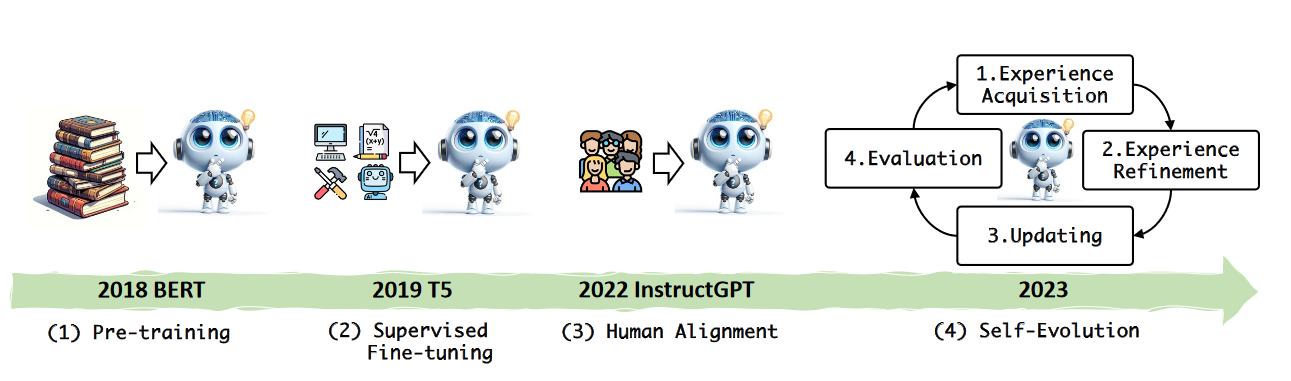
\includegraphics[width=\textwidth]{pic/LLMShift.png}
    \caption{Training paradigms shift of LLMs.\cite{LLMsurvey}}
    \label{fig:my_label}
\end{figure}
\end{frame}

\begin{frame}{Self-Evolution of LLMs}
There are fundamental abilities to be evolved.\cite{LLMsurvey}
For \textbf{LLMs}:
\begin{itemize}
    \item Reasoning
    \item Math
    \item Role-Play
    \item Others
\end{itemize}
For \textbf{LLM-based Agents}:
\begin{itemize}
    \item Planning
    \item Tool Use
    \item Embodied Control
    \item Communication
\end{itemize}
Can self-evolution of LLMs optimize their own architectures?
\end{frame}

\begin{frame}{Self-Evolution of LLMs}
Problems to be solved:
\begin{itemize}
    \item \textbf{Multi-objective} self-evolution, current methods focus mainly on the single objective.
    \item It is a challenge whether multiple models can \textbf{evolve cooperatively}.
    \item \textbf{The degree of autonomy} of model self-evolution.
    \item The lack of theoretical foundations for \textbf{empirical acquisition} and \textbf{refinement} of models.
    \item The need for more dynamic, comprehensive \textbf{benchmarks} for the evaluation of self-evolving models.
\end{itemize}
\end{frame}

\begin{frame}{Self-Evolution of LLMs}
Some research methods:
\begin{itemize}
    \item Reinforcement learning, AgentGym\cite{agentgym}
    \item Meta-learning
    \item Evolutionary algorithm, evolve the architecture or parameters.
    \item Co-evolution between models.
\end{itemize}
\begin{figure}
    \centering
    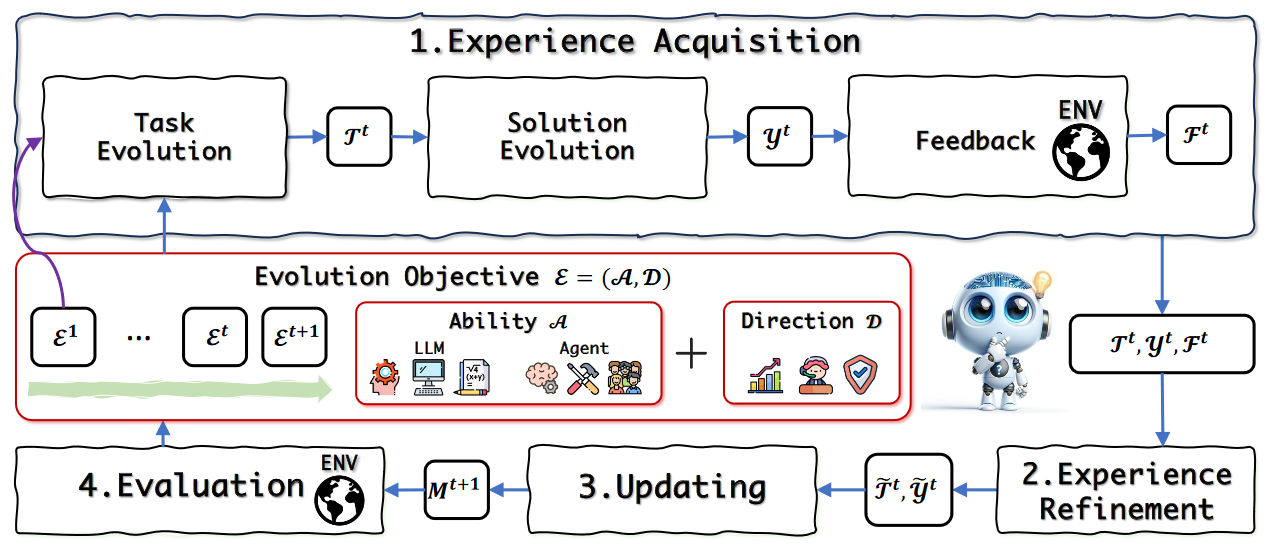
\includegraphics[width=0.9\textwidth]{pic/frameLLM.png}
    \caption{Conceptual framework of self-evolution.\cite{LLMsurvey}}
    \label{fig:my_label}
\end{figure}
\end{frame}

\begin{frame}{Self-Evolution of LLMs}
In the future, I hope through this work, the LLMs can:
\begin{itemize}
    \item have more optimized architecture and performance
    \item have stronger \textbf{generalization ability} and \textbf{multi-task learning ability}
    \item discover and repair their own shortcomings, acquire \textbf{high-quality knowledge} by themselves in dynamic environments
\end{itemize}
\end{frame}



\begin{frame}[standout]
  THANK YOU !
\end{frame}

\metroset{sectionpage=none}
\begin{frame}[allowframebreaks, noframenumbering]{References}
\printbibliography
\end{frame}


\end{document}
